% sections/04-results.tex

\section{Results}\label{sec:results}

We evaluate the eight energy functionals on the first known
counterexamples to Conjecture~\ref{conj:55}, identified via exhaustive enumeration at $n = 9$.

\subsection{Counterexample Data}\label{sec:ce-data}

Two planar triangulations on 9 vertices contain all 48
counterexample colorings:

\begin{table}[htbp]
\centering
\caption{Summary of the two counterexample triangulations at $n = 9$.
  Here $v$ is the removed vertex, CE denotes counterexample colorings,
  $d_{\mathrm{opt}}$ is the optimal BFS distance to a 4-coloring,
  and $d_{\mathrm{safe}}$ is the shortest safe distance.}
\label{tab:ce-summary}
\begin{tabular}{lcccccc}
\toprule
Graph & $v$ & $\deg(v)$ & CE colorings & $d_{\mathrm{opt}}$ &
  $d_{\mathrm{safe}}$ & $d_{\mathrm{safe}} - d_{\mathrm{opt}}$ \\
\midrule
$T_{9,25}$ & 3 & 5 & 24 & 2 & 3 & 1 \\
$T_{9,35}$ & 6 & 4 & 24 & 2 & 3 & 1 \\
\bottomrule
\end{tabular}
\end{table}

In both cases, the detour cost is exactly one additional Kempe swap.
Every counterexample coloring has at least one safe path of length 3,
consistent with Conjecture~\ref{conj:55prime}.

\begin{figure}[htbp]
\centering
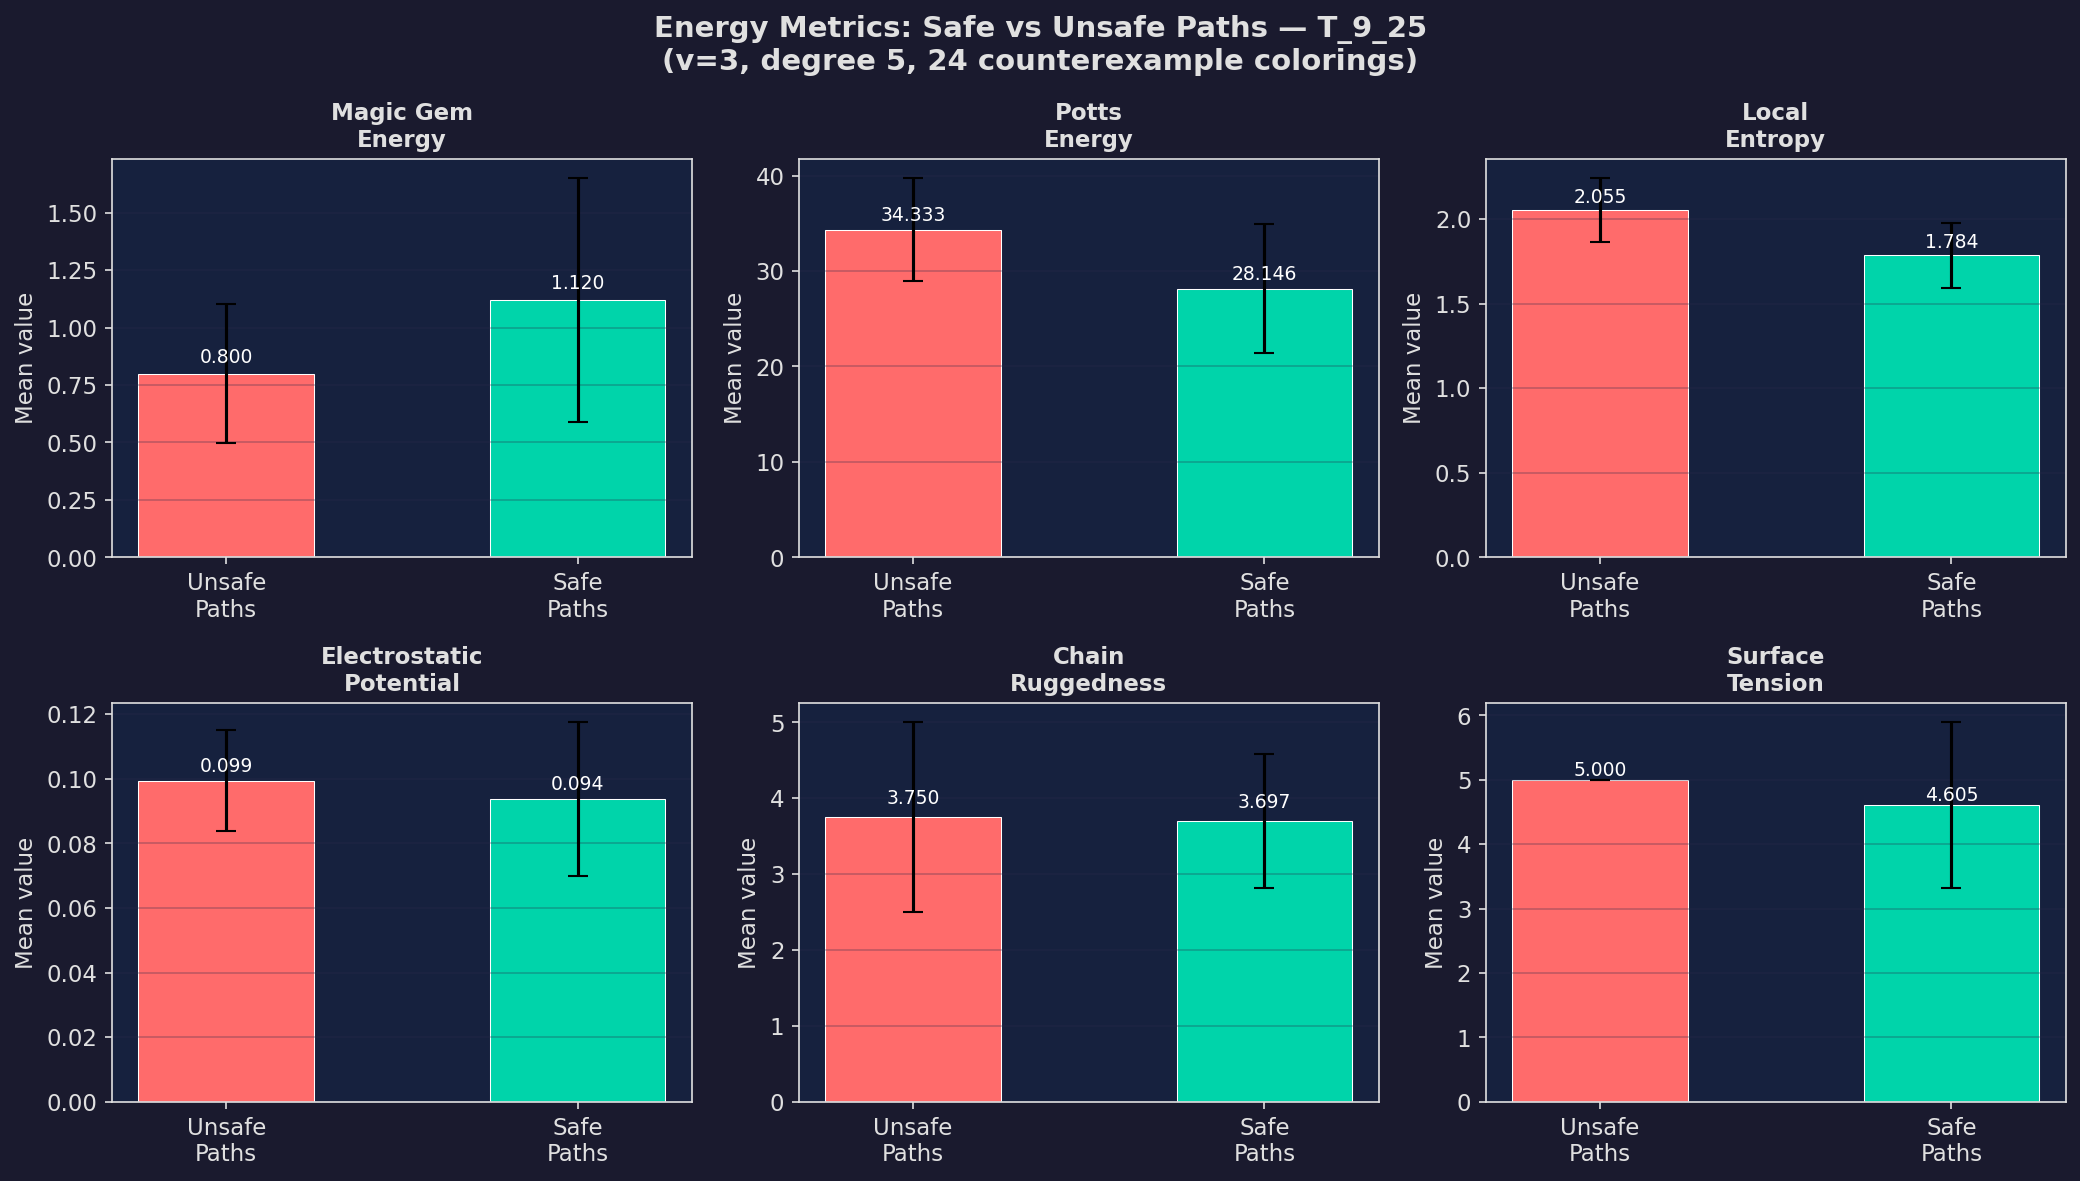
\includegraphics[width=\textwidth]{figures/safe_vs_unsafe_energy_bars_T_9_25.png}
\caption{Energy functional values for safe versus unsafe first-step
  swaps in $T_{9,25}$. Each bar represents one Kempe swap from a
  counterexample coloring; blue bars are safe swaps, red bars are
  unsafe. Among the eight functionals, local entropy and Magic Gem
  energy show the largest separation between safe and unsafe
  distributions.}
\label{fig:safe-unsafe-bars}
\end{figure}

\subsection{Discriminating Metrics}\label{sec:discriminating}

\paragraph{Local Entropy.}
The local entropy $S(v, c)$ at the critical vertex $v$ provides the
strongest discrimination between safe and unsafe paths among the eight
functionals tested (see Figure~\ref{fig:safe-unsafe-bars}).
For $T_{9,25}$ (averaged over all 24 counterexample colorings):
\begin{align}
  \bar{S}_{\text{unsafe}} &= 2.055, \label{eq:entropy-unsafe} \\
  \bar{S}_{\text{safe}} &= 1.784, \label{eq:entropy-safe} \\
  \Delta S &= +0.271. \label{eq:entropy-delta}
\end{align}
(These are means; we do not report per-coloring variance here, though
visual inspection of Figure~\ref{fig:safe-unsafe-bars} shows the
distributions are well-separated.)
Unsafe swaps lead to colorings with \emph{higher} local entropy,
more uniformly distributed neighbor colors, which counterintuitively
reduces the structural diversity needed to maintain chain separation.
Intuitively, high entropy means no color dominates the neighborhood,
making it easier for chains of different color pairs to merge.

\paragraph{Magic Gem Trajectory.}
The global Magic Gem energy $E_{\mathrm{MG}}(G, c)$ (dimensionless;
defined in Section~\ref{sec:mg-energy}) along reconfiguration paths
reveals qualitatively different trajectory shapes.  The following values
are for a single representative counterexample coloring in $T_{9,25}$:
\begin{itemize}
  \item \textbf{Unsafe trajectory} (greedy descent then barrier):
    $0.619 \to 0.556 \to 1.224$. The first step decreases energy
    by $0.063$, but the second step encounters a barrier of $+0.668$
    as the merge-prone chain is forced.
  \item \textbf{Safe trajectory} (ridge then non-monotone):
    $0.619 \to 1.481 \to 1.077 \to 1.992$. The first step
    \emph{increases} energy by $0.862$ (crossing a ridge), the second
    decreases it by $0.404$, and the third reaches the 4-coloring at
    $E_{\mathrm{MG}} = 1.992$. No merge-prone swaps are encountered
    along this path.
\end{itemize}
The ridge height at the first step is the key distinguishing feature.

\paragraph{Surface Tension Rigidity.}
Across all 48 counterexample colorings at $n = 9$, unsafe Kempe chains
exhibit \emph{zero variance} in their normalized surface tension:
\begin{equation}\label{eq:st-zero}
  \Gamma_{ab}(c_{\text{unsafe}}) = 0,
  \qquad
  \Gamma_{ab}(c_{\text{safe}}) > 0.
\end{equation}
All chains in the merge-prone color pair have identical boundary-to-size
ratios, indicating a rigid configuration with no structural variability. Safe
chains, by contrast, exhibit variable tension — some are compact with
low boundary cost, others are elongated with high boundary cost — giving
the reconfiguration process more degrees of freedom to avoid merges.

\begin{figure}[htbp]
\centering
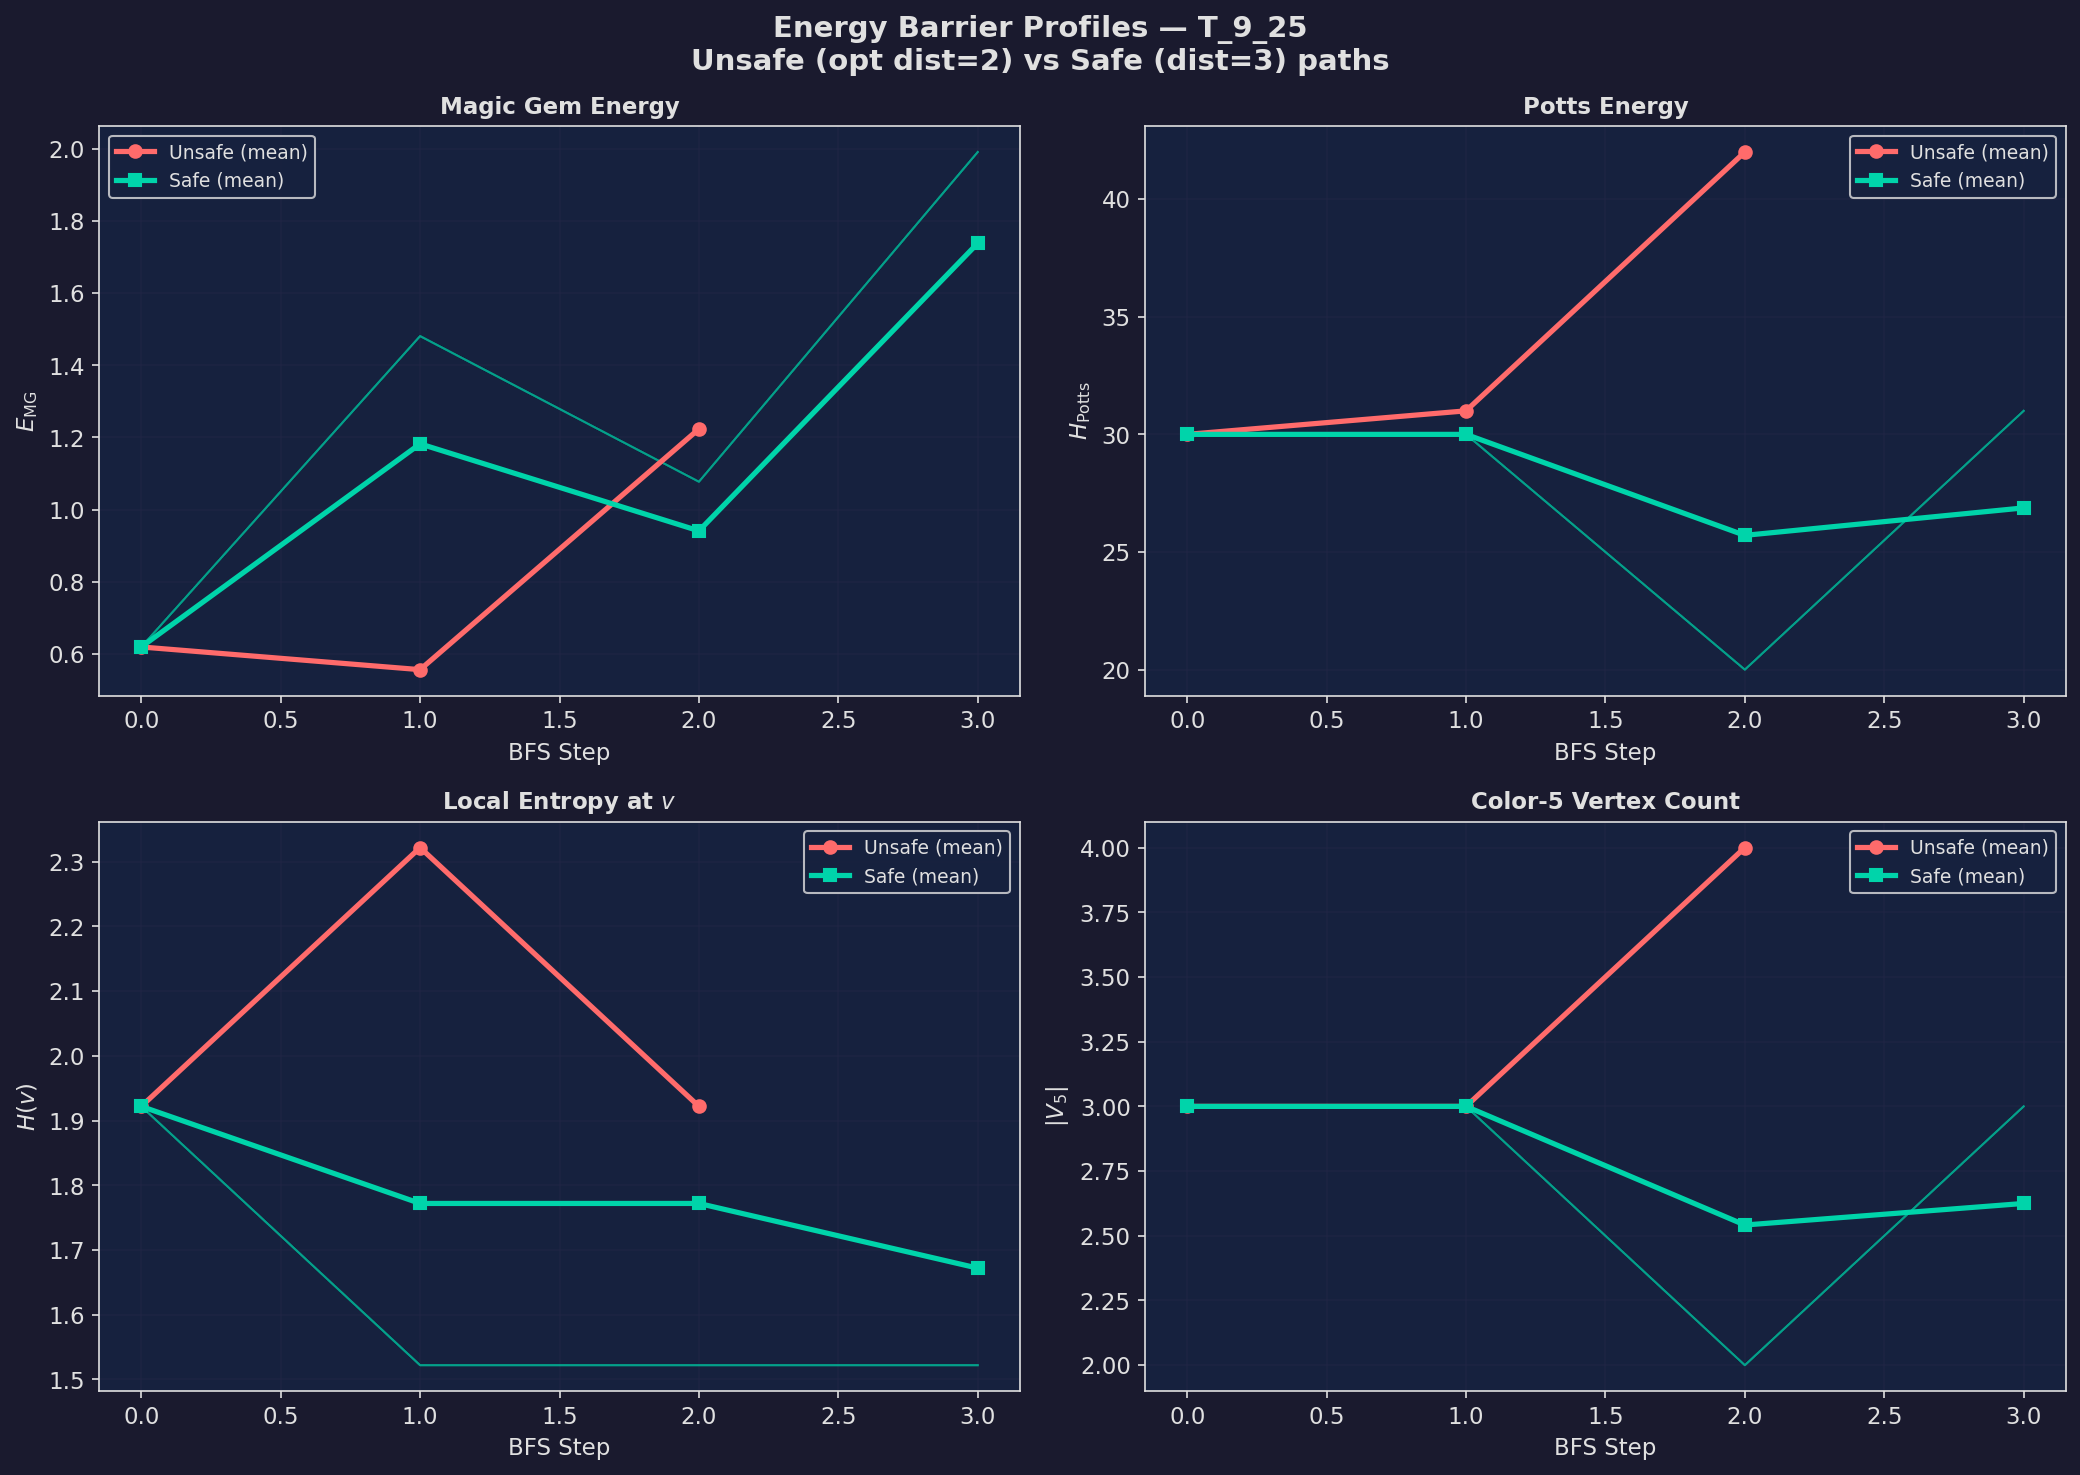
\includegraphics[width=\textwidth]{figures/energy_barrier_profile_T_9_25.png}
\caption{Energy barrier profile along optimal (unsafe, red) and safe
  (blue) reconfiguration paths for a representative counterexample
  coloring in $T_{9,25}$. The Magic Gem energy is plotted at each step.
  The safe path crosses a ridge at step~1 that the optimal path avoids,
  but the optimal path encounters a merge barrier at step~2.}
\label{fig:energy-barrier}
\end{figure}

\subsection{The Kinetic Trap Structure}\label{sec:kinetic-trap}

The reconfiguration landscape near each counterexample exhibits a
two-basin structure:

\begin{description}
  \item[Basin A (unsafe):] Reached by greedy descent in
    $E_{\mathrm{MG}}$. The first Kempe swap reduces the Magic Gem
    energy, but the resulting coloring has merge-prone chains. All
    continuations to a 4-coloring from this basin require traversing
    an unsafe swap.
  \item[Basin B (safe):] Accessed by crossing an energy ridge at the
    first step. The initial swap \emph{increases} $E_{\mathrm{MG}}$ by
    $\Delta E_{\mathrm{MG}} = 0.862$ for $T_{9,25}$ and $0.96$ for
    $T_{9,35}$ (each computed from a representative counterexample
    coloring; only the $T_{9,25}$ trajectory is shown in full above). From Basin~B, all paths
    to a 4-coloring avoid merges.
\end{description}

This structure is analogous to protein folding kinetic
traps~\cite{levinthal1969}: Basin~A is a misfolded state reached by
greedy energy minimization, while Basin~B is the native fold reached by
a thermodynamically less favorable but kinetically accessible pathway.

\begin{figure}[htbp]
\centering
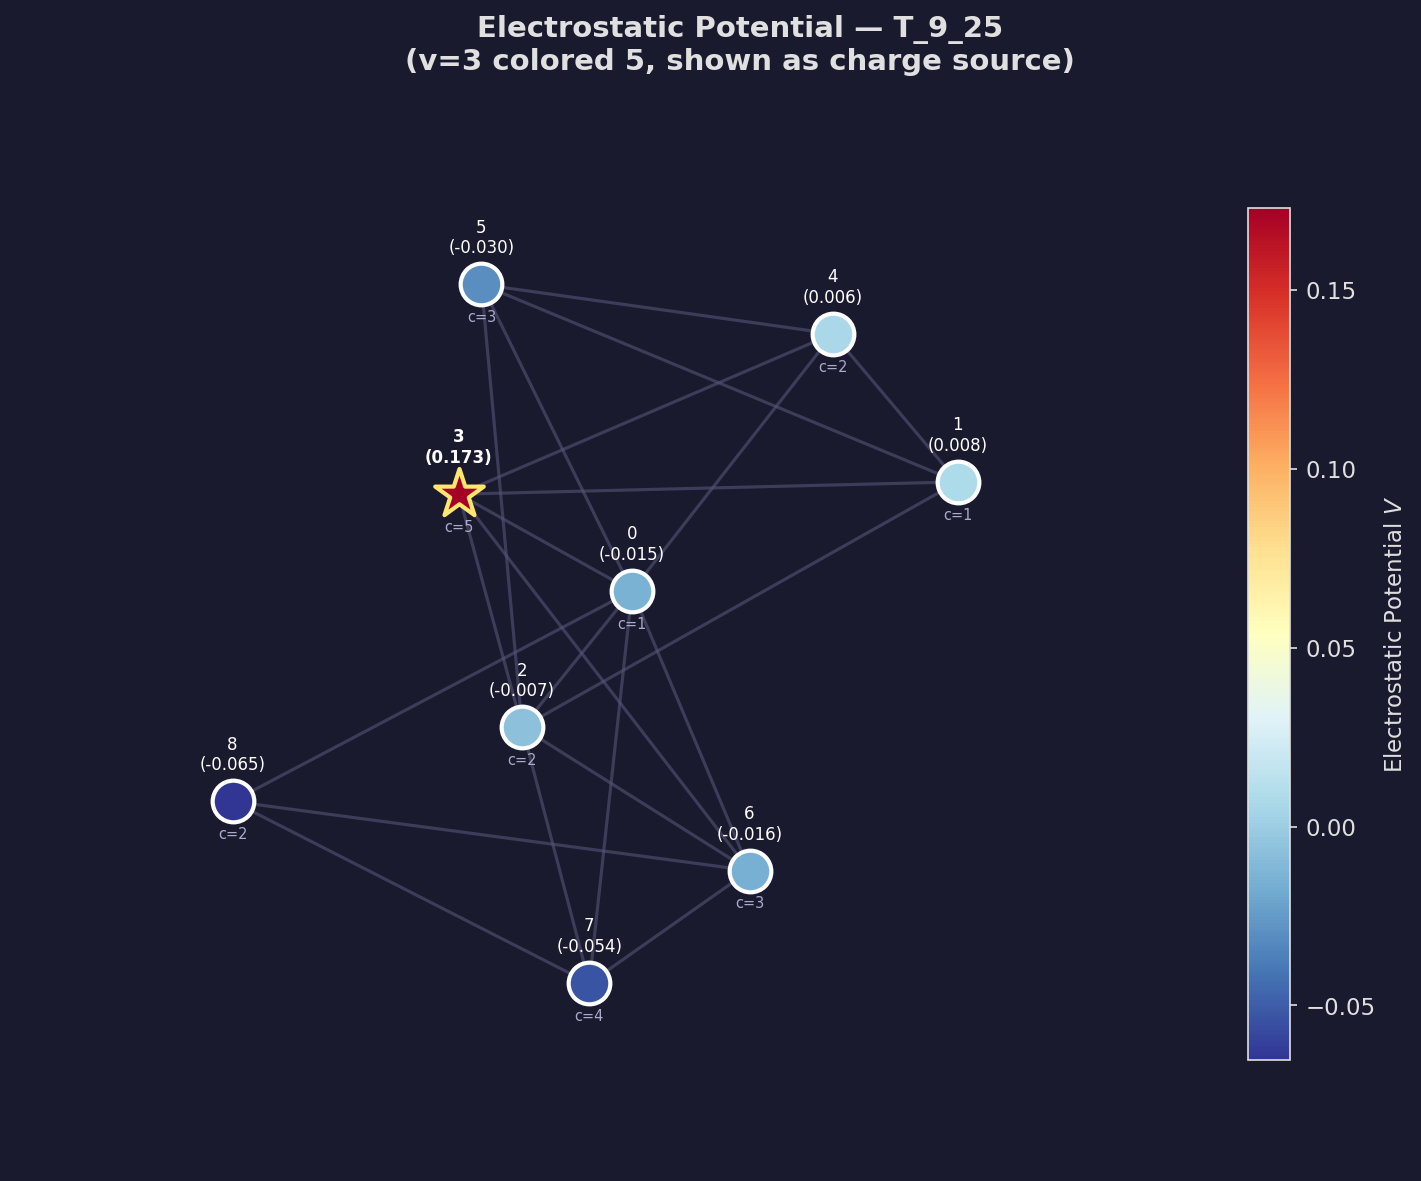
\includegraphics[width=\textwidth]{figures/electrostatic_heatmap_T_9_25.png}
\caption{Electrostatic potential heatmap for a counterexample coloring
  of $T_{9,25}$. Vertices colored 5 (defects) appear as charge sources.
  The potential gradient is highest at the boundary between the critical
  vertex's neighborhood and the rest of the graph.}
\label{fig:electrostatic}
\end{figure}

\subsection{The Surface Tension Rigidity Conjecture}
\label{sec:st-conjecture}

The computational evidence at $n = 9$ motivated the following conjecture.

\begin{conjecture}[Surface Tension Rigidity]\label{conj:st-rigidity}
Let $G$ be a planar triangulation, $c$ a proper 5-coloring of $G$,
$v$ a vertex, and $(a,b)$ a color pair such that the Kempe
$(a,b)$-swap is the first step of a reconfiguration path from $c$
toward a 4-coloring. If the surface tension rigidity
$\Gamma_{ab}(c) = 0$ — that is, all Kempe $(a,b)$-chains have identical
normalized surface tension — then the swap merges two chains incident
to $v$ (i.e., the swap is unsafe).
\end{conjecture}

\begin{remark}[Subsequent falsification]\label{rem:st-falsified}
Conjecture~\ref{conj:st-rigidity} was falsified by exhaustive
computation at $n \geq 10$: instances with $\Gamma_{ab} = 0$ for safe
swaps were identified (the exact count has not been tabulated, but at
least several dozen such instances exist), violating the conjecture's
implication. While the
implication $\Gamma_{ab} = 0 \implies \text{unsafe}$ holds for all 48
counterexamples at $n = 9$, it does not generalize to $n \geq 10$. The
conjecture is retained here as part of the intellectual record; the
local entropy and kinetic trap signatures
(Sections~\ref{sec:discriminating}--\ref{sec:kinetic-trap}) continue to
hold in the extended dataset.
\end{remark}

\begin{remark}\label{rem:converse}
The converse does not hold in general: some unsafe swaps have
$\Gamma_{ab}(c) > 0$. However, within the 48 counterexamples at $n = 9$,
zero rigidity is a \emph{sufficient} condition for unsafety.
\end{remark}

\paragraph{Evidence at $n = 9$.}
Across all 48 counterexample colorings (24 in $T_{9,25}$, 24 in
$T_{9,35}$) at $n = 9$, every unsafe first-step swap has
$\Gamma_{ab} = 0$, while every safe first-step swap has
$\Gamma_{ab} > 0$. The effect is consistent across both triangulations
despite their different local structures
($\deg(v) = 5$ vs.\ $\deg(v) = 4$). As noted in
Remark~\ref{rem:st-falsified}, this pattern does not persist at
larger scales.
